\documentclass[11pt,a4paper]{ivoa}
\usepackage[margin=4.25cm]{geometry} 
\usepackage{longtable}
\input tthdefs
\setcounter{tocdepth}{2}

\title{Astronomical Coordinates and Coordinate Systems}

% see ivoatexDoc for what group names to use here
\ivoagroup{Data Model Working Group}

%\author[????URL????]{????Alfred Usher Thor????}
\author{Arnold Rots}
\author{Mark Cresitello-Dittmar}
\author{Omar Laurino}
\author{Test}

\editor{Arnold Rots}
\editor{Mark Cresitello-Dittmar}

% \previousversion[????URL????]{????Funny Label????}
\previousversion{This is the first public release}
       
\begin{document}
\begin{abstract}
  In creating version 2 of the ``Space-Time Coordinate Metadata for the Virtual Observatory'' (STC) Data Model \citep{std:STC}, it was decided to split the content into various component models which focus on particular aspects of the previous model scope.  
  
  This model describes the Coordinates model and covers the following concepts.
  \begin{itemize}
  \item Description of single and multi-dimensional coordinate space, and coordinates within that space.
  \item Coordinate Frames, providing metadata describing the origin and orientation of the coordinate space.
  \item Definition of simple domain-specific coordinate types for the most common use cases.
  \item Coordinate Systems, description of the coordinate domain space.
  \end{itemize}
\end{abstract}


\section*{Acknowledgments}
This document has been developed with support from NSF and NASA under the Virtual Astronomical Observatory (VAO) project, the National Science Foundation’s (\url{http://www.nsf.gov}) Information Technology Research Program under Cooperative Agreement AST0122449 with The Johns Hopkins University, from the UK Particle Physics and Astronomy Research Council (PPARC),\url{http://www.pparc.ac.uk}, and from the Euro-VO projects (European Commission 7th program): Euro-VO Aida, VO-ICE and CoSADIE.

\section*{Conformance-related definitions}

The words ``MUST'', ``SHALL'', ``SHOULD'', ``MAY'', ``RECOMMENDED'', and
``OPTIONAL'' (in upper or lower case) used in this document are to be
interpreted as described in IETF standard RFC2119 \citep{std:RFC2119}.

The \emph{Virtual Observatory (VO)} is a
general term for a collection of federated resources that can be used
to conduct astronomical research, education, and outreach.
The \href{http://www.ivoa.net}{International
Virtual Observatory Alliance (IVOA)} is a global
collaboration of separately funded projects to develop standards and
infrastructure that enable VO applications.


\newgeometry{left=1.0in,right=1.0in,bottom=1.0in}
\section{Introduction}

\subsection{Motivation}
Astronomy, being primarily a science that crucially depends on observations, has a very basic 
need for complete, accurate, and unambiguous metadata regarding coordinate information, meaning 
all coordinates of the observable space and noting that several of these are intertwined. The Data 
Model described in this document aims to provide a model for such metadata.

\subsection{Context and Scope}
This document results from updating the \href{http://www.ivoa.net/documents/latest/STC.html}{``Space-Time Coordinate Metadata for the Virtual Observatory''} (STC) \citep{std:STC} model for use in VO-DML compliant models. That model provides metadata describing Space-Time related, and other Coordinates. These metadata are to be used for specifying coordinate-related information for datasets, catalogs, and queries.  In this work, our primary focus is to support the use cases described below, while keeping the broader scope in mind to inform design decisions for future expansion.

The update and revision of the STC model has sub-divided the content into component models, each covering a portion of the scope of the parent model.  This allows for a better description of the relations between the various components, allows for independent development of the component models, and creates smaller, more digestible content for users.

In the astronomical community, the terms ``quantity'', ``coordinate'', and ``measurement'' are used interchangably, but not always 
with the same meaning.  The ``coordinate'' of a star is typically a measured location, while the ``coordinate'' of the center
of a circular region is not.  We provide here a short glossary of these terms in the IVOA data model context.
\begin{itemize}
  \item Quantity: [ivoa model]  A number with a unit.
  \item Coordinate: [coords model]  An absolute location within a coordinate space.  Comprised of a 'value' (often a Quantity), 
associated with an axis in a coordinate space, and a coordinate frame providing additional metadata about the orientation and origin of the coordinate space.
In other words, a location in a domain space.
  \item Measurement: [meas model]  For 'measured', or 'determined' data.  Combines a Coordinate (ie: the determined value) with 
corresponding Error(s).  For the majority of cases dealing with astronomical data, this is what we are referring to.
  \item Coordinate System: [coords model]  The term 'Coordinate System' is used to mean both ``the space in which a coordinate resides'', and ``a unique domain space, factoring in specific reference frame metadata''.  In this model, we adopt the latter definition.  A Coordinate System provides a complete description of the domain space, including both the coordinate space description and any associated Frame metadata.
\end{itemize}

This document describes the Coordinates model which provides the metadata describing:
\begin{itemize}
\item the coordinate space; axes, and domain ranges
\item coordinate frames with metadata describing the origin and orientation of the coordinate space
\item a general model for specifying coordinate values within the coordinate space
\item coordinate systems for defining various domain spaces.
\end{itemize}

\section{Use Cases and Requirements}
\label{sect:ucreq}

\subsection{Use Cases}
\label{sect:usecases}

\subsubsection{Cube model support}
\label{uc:Cube-model-support}
  The primary use case for this work is in support of the CubeDM. \\
  The CubeDM is a N-Dimensional model for pixelated images and sparse cube data.  
  The following is a brief outline of the most relevant features pertaining to the
  development of the Measurement, Coordinates, and Transform component models.

  \begin{itemize}
    \item General
    \begin{itemize}
       \item knowledge of the pixel and physical domain spaces provided at a high level
       \item definition of the domain space includes the following criteria
       \begin{itemize}
          \item dimensionality (typically 1,2 or 3 for physical domain), pixel domain may be of any dimension
          \item axis configuration (for spatial domain which has >1D).  The most common configurations for astronomical data are Cartesian and Spherical, but others may be used as well.
          \item domain range along each axis, typically +/- Inf, but may be limited due to physical constraints (e.g. physical size of a detector, sensitivity limitiations, etc)
          \item association with additional metadata further describing the nature of the domain space ( Frame ).  This is especially true for the Spatial and Temporal domains, but may apply to others as well.  Examples include:
          \begin{itemize}
             \item reference position (location of origin)
             \item reference frame (orientation of the domain space)
             \item planetary ephemeris
             \item equinox
          \end{itemize}
       \end{itemize}
    \end{itemize}
    \item Pixelated Image Cube
    \begin{itemize}
       \item complete specification of pixel coordinate domain; number of axes, number of pixels per axis
       \item mappings of various pixel axes to corresponding physical axes
       \begin{itemize}
          \item spatial domain typically mapping 2-3 pixel axes to physical axes
          \item other domains are typically 1 dimensional
          \item pixel axes may be involved in multiple mappings to different physical spaces
        \end{itemize}
        \item mappings may be stacked to define progressive transitions through a domain (e.g.:  pixel -> ccd -> detector -> sky -> wcs )
        \begin{itemize}
           \item intermediate stages may or may not be explicitely defined 
        \end{itemize}
        \item image data value is typically given in a physical domain, but may itself be mapped to other domains
    \end{itemize}
    \item Sparse Cube
    \begin{itemize}
       \item data axes cover a wide array of physical domains including, but not limited to Spatial, Temporal, Spectral, Polarization,
       \item individual domains may be represented multiple times in different frames ( ccd, detector, sky;  pha, energy )
       \item data values may have associated errors
       \begin{itemize}
          \item typical error forms include: symmetric( +/- a ), asymmetric( +a:-b ), interval ( a:b ), matrix, elliptical
          \item can become quite complex: probability distributions, error maps, etc.
          \item quality indicators:
          \begin{itemize}
             \item global status, typically numeric
             \item bit array, where each bit is associated with a particular quality state 
          \end{itemize}
          \item associated errors may be separable or correlated among multiple data axes
        \end{itemize}
        \item data axes may be virtual, defined as a mapping from other data axes (same description as above)
    \end{itemize}
    \item Physical Data (Observables)
    \begin{itemize}
       \item focus on the following domains which are frequently included in astronomical data cubes: Spatial, Spectral, Temporal, Polarization
       \item Spatial
       \begin{itemize}
          \item Cartesian space:  chip, detector, sky
          \item Spherical space: Equatorial, Ecliptic, Galactic, LongLat
       \end{itemize}
       \item Time
       \begin{itemize}
          \item 1-Dimensional: JD, MJD, ISOTime, TimeOffset
       \end{itemize}
       \item Polarization
       \begin{itemize}
          \item Discrete space: Polarization states (Stokes, Linear, Circular, Vector )
       \end{itemize}
       \item Spectral
       \begin{itemize}
          \item 1-Dimensional: energy, frequency, wavelength
       \end{itemize}
    \end{itemize}
  \end{itemize}

\subsubsection{Transform workflow}
\label{uc:Transform-workflow}
An implementation project focused on the Transform model. The purpose of which is to exercise the Transform model through a workflow consisting of:
  \begin{itemize}
    \item serialization in YAML of complete WCS metadata, including source/target frames and the various Transform operation sequences between them.
    \item the generation and passing thereof between two Transform library implementations ( AST, gWCS )
  \end{itemize}


\subsection{Requirements}
\label{sect:reqs}

 Examination and implementation of the above cases leads to a set of requirements distributed through the various STC component models.  Here we 
itemize those relevant to the coordinates model specifically.  We note that some elements of this model are included based on the knowledge and 
experience incorporated into previous STC data model and not from direct requirements from the given use cases.  

In Appendix \ref{sect:req_map}, we provide a mapping of the data model elements to the various requirements they serve.

\subsubsection{General}
Requirements pertaining to the overall criteria that the model must satisfy.
  \begin{itemize}
    \item [\textbf{[vodml.001]:}] The model shall be vo-dml compliant
    \item [\textbf{[vodml.002]:}] shall re-use, or refer to, dependent models for objects and concepts already defined in other models
    \item [\textbf{[vodml.003]:}] shall produce a validated vo-dml XML description
    \item [\textbf{[vodml.004]:}] shall produce documentation in vo-dml HTML format
    \item [\textbf{[vodml.005]:}] shall produce documentation in standard PDF format
  \end{itemize}

\subsubsection{Application/Usage}
Requirements pertaining to the user experience.  Note, as a data model, users will not typically interact directly with the model,
  \begin{itemize}
    \item [\textbf{[user.001]:}] Users should be able to identify and use basic content with minimal specialized information. 
      In other words, a generic utility should be able to find and use core elements without knowing a lot about the various extensions and uses of those elements.
    \item [\textbf{[user.002]:}] When applicable, the model should support usability by simplifying common scenarios. i.e. common things simple, complex things possible
  \end{itemize}

\subsubsection{Content}
Requirements pertaining to the elements to be defined by the model.
\begin{itemize}
  \item Domains
  \begin{itemize}
    \item [\textbf{[dom.001]:}] Shall accommodate the description of data in any observable domain
    \item [\textbf{[dom.002]:}] Shall provide enhanced/specialized description for data pertaining to
    \begin{itemize}
      \item [\textbf{[dom.002.1]:}] Pixel domain: binned, integerized, n-dimensional domain
      \item [\textbf{[dom.002.2]:}] Spatial domain: continuous domain, typically in 2-3 dimensional cartesian or spherical spaces
      \item [\textbf{[dom.002.3]:}] Time domain: continuous 1D domain, typically provided in JD, MJD, ISO, or as an Offset from a zero point
      \item [\textbf{[dom.002.4]:}] Polarization domain: discrete 1D domain of polarization states. 
    \end{itemize}
  \end{itemize}
  \item Coordinates
  \begin{itemize}
    \item Coordinate Spaces:
    \begin{itemize}
      \item [\textbf{[coords.001]:}] Shall facilitate the description of the domain space
      \begin{itemize}
        \item [\textbf{[coords.001.1]:}] Coordinate space shall consist of 1 to N dimensional axes
        \item [\textbf{[coords.001.2]:}] Shall support the description of axes which are continuous, binned, and discrete in nature
        \item [\textbf{[coords.001.3]:}] Each dimensional axis shall define the domain range of that axis as appropriate for its nature
      \end{itemize}
    \end{itemize}
    \item Coordinate frames: 
    \begin{itemize}
      \item [\textbf{[coords.002]:}] Shall facilitate the specification of the nature of the domain, providing additional metadata relevant to the interpretation of coordinates in that domain.
    \end{itemize}
    \item Coordinates: 
    \begin{itemize}
      \item [\textbf{[coords.003]:}] Shall identify a location within the coordinate domain space
      \item [\textbf{[coords.004]:}] Shall be associated with a corresponding coordinate frame providing metadata relevant to the interpretation of the coordinate
      \item [\textbf{[coords.005]:}] Shall be associated with a particular axis of the coordinate space to provide context for the coordinate and facilitate the application of mapping Transforms
      \item [\textbf{[coords.006]:}] Shall be complete quantities, including value and units as appropriate
      \item [\textbf{[coords.007]:}] Shall support the association of atomic coordinates into a multi-dimensional compound grouping
    \end{itemize}
    \item Coordinate systems: 
    \begin{itemize}
      \item [\textbf{[coords.008]:}] Shall provide for encapsulating the description of the entire domain space
      \item [\textbf{[coords.009]:}] for Pixel domain, this must include the full coordinate space description
      \item [\textbf{[coords.010]:}] for Physical domains, this must include the Frame specifications, as it is this metadata that is more relevant to users.  The coordinate space is typically well defined or implied by the coordinate itself.
    \end{itemize}
  \end{itemize}

  \item Transforms
  \begin{itemize}
    \item [\textbf{[trans.001]:}] Shall facilitate the relation of two coordinate systems through a mathematical formula (Transforms)
    \begin{itemize}
      \item [\textbf{[trans.001.1]:}] Shall facilitate the transport of same independent of any actual data.
    \end{itemize}
  \end{itemize}

\end{itemize}


\pagebreak
\subsection{Role within the VO Architecture}

\begin{figure}[h]
\centering

% As of ivoatex 1.2, the architecture diagram is generated by ivoatex in
% SVG; copy ivoatex/archdiag-full.xml to archdiag.xml and throw out
% all lines not relevant to your standard.
% Notes don't generally need this.  If you don't copy archdiag.xml,
% you must remove archdiag.svg from FIGURES in the Makefile.

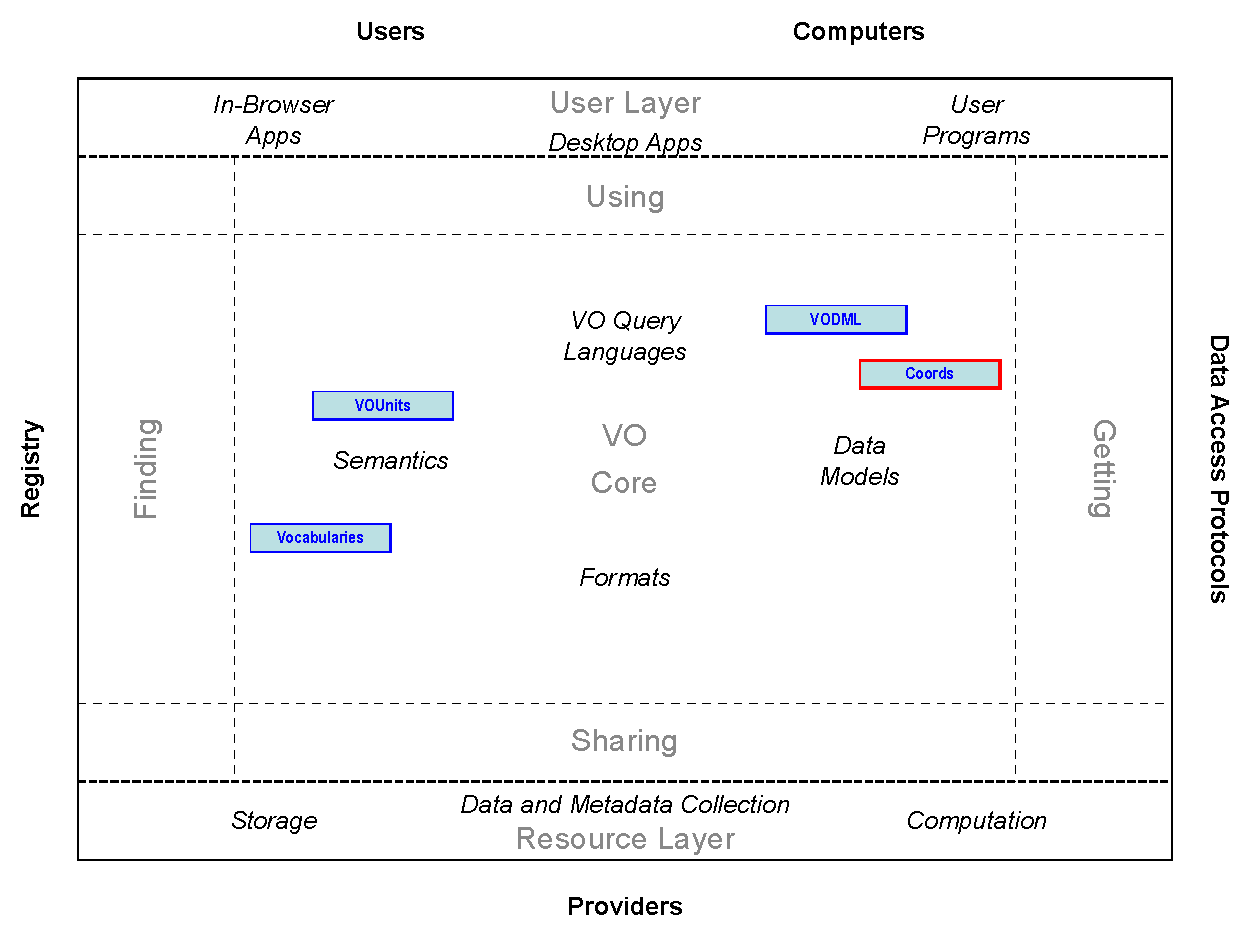
\includegraphics[width=0.9\textwidth]{role_diagram.pdf}
\caption{Architecture diagram for this document}
\label{fig:archdiag}
\end{figure}

Fig.~\ref{fig:archdiag} shows the role this document plays within the
IVOA architecture \citep{note:VOARCH}.


% -------------------------------------------
% Items to substitute into the ivoatex document template.
%
%\ivoagroup{Data Model Working Group}

%\title{Astronomical Coordinates and Coordinate Systems}


%\author{Arnold Rots}
    
%\author{Mark Cresitello-Dittmar}
    
%\author{Omar Laurino}
    
%\previousversion{0}
      
% -------------------------------------------

\pagebreak
\section{Model: coords }
  
  % INSERT FIGURE HERE
  \begin{figure}[h]
  \begin{center}
    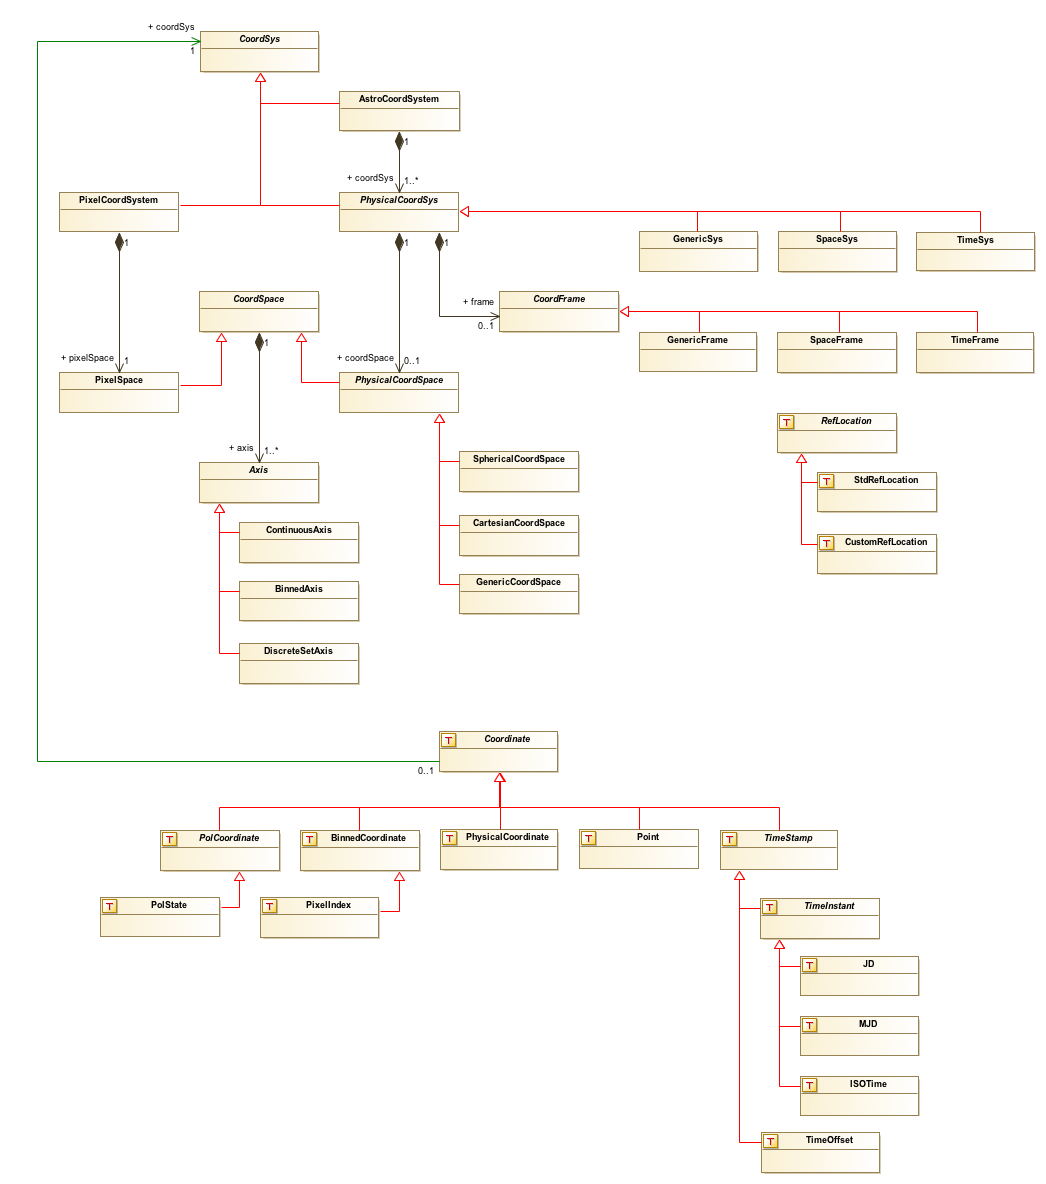
\includegraphics[width=\textwidth]{diagrams/Overview.png}
    \caption{Model Overview}\label{fig:overview}
  \end{center}
  \end{figure}

  This model defines objects which describe the coordinate space, coordinates within that space, and frames, which provide additional metadata regarding the origin, orientation, etc, of the coordinate space. The model also defines a coordinate system, bundling frames into associated groups.

\pagebreak
\section{Coordinates}

  % INSERT FIGURE HERE
  \begin{figure}[h]
  \begin{center}
    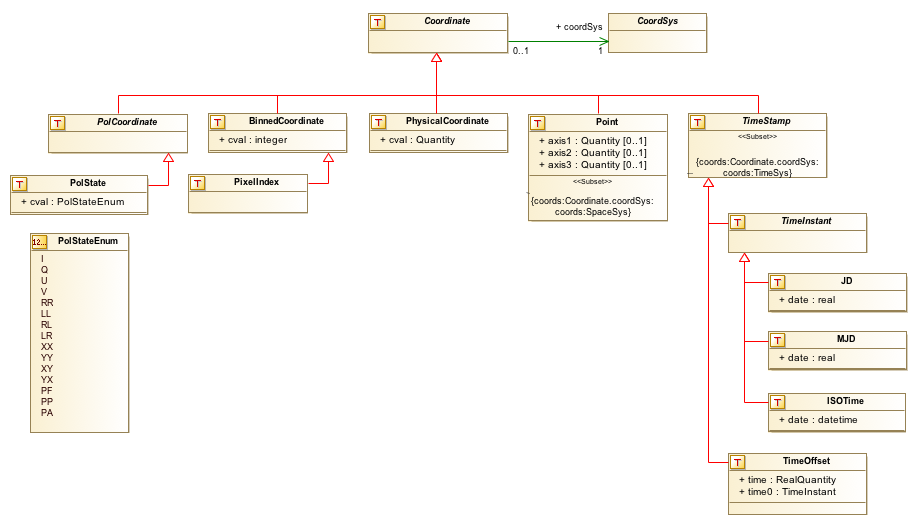
\includegraphics[width=6in]{diagrams/Coordinates.png}
    \caption{Coordinate elements}\label{fig:coordinates}
  \end{center}
  \end{figure}

  This section provides support for the most commonly used coordinate types.  The design allows for the specification of custom coordinate spaces, but leverages the fact that most data will reside in well defined standard spaces.  \textbf{It is expected that these coordinates will be used in the vast majority of cases.}


  \subsection{Coordinate (Abstract)}
  \label{sect:Coordinate}
    Abstract base class for the Coordinate data types which represent an absolute location within a coordinate space. Coordinates MUST refer to a coordinate system, providing additional metadata relevant to interpreting the coordinate value, and its representation.

    \subsubsection{Coordinate.coordSys}
      \textbf{vodml-id: Coordinate.coordSys} \newline
      \textbf{type: \hyperref[sect:CoordSys]{coords:CoordSys}} \newline
      \textbf{multiplicity: 1} \newline 
      Provided additional metadata relevant to interpreting the coordinate value; for example, the spatial reference position, or time scale, axis descriptions.


  \subsection{BinnedCoordinate}
  \label{sect:BinnedCoordinate}
    Coordinate value type specifically intended for binned data (e.g.: pixel indexes).

    \subsubsection{BinnedCoordinate.cval}
      \textbf{vodml-id: BinnedCoordinate.cval} \newline
      \textbf{type: \hyperref[sect:ivoa]{ivoa:integer}} \newline
      \textbf{multiplicity: 1} \newline 
      The binned coordinate value, expressed as an integer. e.g.: bin number, pixel index.


  \subsection{PhysicalCoordinate}
  \label{sect:PhysicalCoordinate}
    The most common type of coordinate value. This type is appropriate for any data whose values can be described by an ivoa:Quantity (numeric, with unit).

    \subsubsection{PhysicalCoordinate.cval}
      \textbf{vodml-id: PhysicalCoordinate.cval} \newline
      \textbf{type: \hyperref[sect:ivoa]{ivoa:Quantity}} \newline
      \textbf{multiplicity: 1} \newline 
      This coordinate MUST contain a value expressed as an ivoa:Quantity.


  \subsection{Point (Abstract)}
  \label{sect:Point}
    Multi-dimensional spatial coordinate. The Point MUST refer to a spatial coordinate system (SpaceSys) which associates the point with corresponding coordinate domain space and frame metadata.

    \noindent \textbf{subset} \newline
    \indent   \textbf{role: coords:Coordinate.coordSys} \newline
    \indent   \textbf{type: coords:SpaceSys} \newline


  \subsection{CartesianPoint}
  \label{sect:CartesianPoint}
    A spatial coordinate in a Cartesian coordinate space. Any associated CoordSpace MUST be a CartesianCoordSpace. If no CoordSpace is provided, a Standard Cartesian CoordSpace is assumed. Values for unused/undefined dimensions need not be provided.

    \subsubsection{CartesianPoint.x}
      \textbf{vodml-id: CartesianPoint.x} \newline
      \textbf{type: \hyperref[sect:ivoa]{ivoa:Quantity}} \newline
      \textbf{multiplicity: 0..1} \newline 
      The coordinate value along the 'X' axis.

    \subsubsection{CartesianPoint.y}
      \textbf{vodml-id: CartesianPoint.y} \newline
      \textbf{type: \hyperref[sect:ivoa]{ivoa:Quantity}} \newline
      \textbf{multiplicity: 0..1} \newline 
      The coordinate value along the 'Y' axis.

    \subsubsection{CartesianPoint.z}
      \textbf{vodml-id: CartesianPoint.z} \newline
      \textbf{type: \hyperref[sect:ivoa]{ivoa:Quantity}} \newline
      \textbf{multiplicity: 0..1} \newline 
      The coordinate value along the 'Z' axis.


  \subsection{LonLatPoint}
  \label{sect:LonLatPoint}
    A spatial coordinate in a Spherical coordinate space defining a Celestial position in Latitude and Longitude. Any associated CoordSpace MUST conform to this description. If no CoordSpace is provided, a Standard Spherical CoordSpace is assumed. Values for unused/undefined dimensions need not be provided.

    \subsubsection{LonLatPoint.lon}
      \textbf{vodml-id: LonLatPoint.lon} \newline
      \textbf{type: \hyperref[sect:ivoa]{ivoa:Quantity}} \newline
      \textbf{multiplicity: 0..1} \newline 
      The longitude of the Point, as a Quantity with angular units.

    \subsubsection{LonLatPoint.lat}
      \textbf{vodml-id: LonLatPoint.lat} \newline
      \textbf{type: \hyperref[sect:ivoa]{ivoa:Quantity}} \newline
      \textbf{multiplicity: 0..1} \newline 
      The latitude of the Point, as a Quantity with angular units.

    \subsubsection{LonLatPoint.dist}
      \textbf{vodml-id: LonLatPoint.dist} \newline
      \textbf{type: \hyperref[sect:ivoa]{ivoa:Quantity}} \newline
      \textbf{multiplicity: 0..1} \newline 
      The distance to the Point from the origin.


  \subsection{GenericPoint}
  \label{sect:GenericPoint}
    GenericPoint supports the representation of spatial coordinates in a custom coordinate space, or any space which is not covered by the other specializations. The coordinate values map, in order, to the axes described by the associated CoordSpace. If no CoordSpace is provided, the behavior is undefined. Values for unused/undefined dimensions need not be provided.

    \subsubsection{GenericPoint.axis1}
      \textbf{vodml-id: GenericPoint.axis1} \newline
      \textbf{type: \hyperref[sect:ivoa]{ivoa:Quantity}} \newline
      \textbf{multiplicity: 0..1} \newline 
      Coordinate value along the first axis of the associated coordinate space, expressed as an ivoa:Quantity.

    \subsubsection{GenericPoint.axis2}
      \textbf{vodml-id: GenericPoint.axis2} \newline
      \textbf{type: \hyperref[sect:ivoa]{ivoa:Quantity}} \newline
      \textbf{multiplicity: 0..1} \newline 
      Coordinate value along the second axis of the associated coordinate space, expressed as an ivoa:Quantity.

    \subsubsection{GenericPoint.axis3}
      \textbf{vodml-id: GenericPoint.axis3} \newline
      \textbf{type: \hyperref[sect:ivoa]{ivoa:Quantity}} \newline
      \textbf{multiplicity: 0..1} \newline 
      Coordinate value along the third axis of the associated coordinate space, expressed as an ivoa:Quantity.


  \subsection{TimeStamp (Abstract)}
  \label{sect:TimeStamp}
    This is the abstract basis for a set of simple time domain coordinates which are expected to accommodate the vast majority of use cases. All TimeStamps, by definition, exist in a standard 1-D coordinate space, with domainMin|Max of +/-Infinity. All TimeStamps MUST refer to an appropriate TimeSys.

    A Brief Primer on Time Metadata; for reference and more information, see: FITS WCS Paper IV \citep{2015A+A...574A..36R}.
    \begin{enumerate}
    \item  Required:\newline
     * Record time stamps in JD, MJD, ISO-8601, or elapsed time. If in elapsed time, a zero point MUST be given in a time stamp which is not itself an elapsed time. \newline
     * Provide the time scale used (e.g. TT, TDB, TAI, GPS, ET, UTC, TCG, TCB). \newline
     * Provide the reference position (place where the time is measured).
    \item  Note the following:  \newline
     * JD and MJD are dimensionless, though a unit of 'day' is implied.  \newline
     * JD and MJD do not imply a time scale; it needs to be provided separately.  \newline
     * JD and MJD are not recommended for expressing times in UTC since not all UTC days are the same length.  Instead, UTC times are best expressed as a formatted string such as the ISOTime type described in Section \ref{sect:ISOTime}. \newline
     * TDB runs on average synchronously with TT, but corrects for the relativistic effects caused by deviations in the orbit of the Earth from perfect circularity and constant gravitational potential. \newline
    \item Recommendations:  \newline
     * Avoid UTC. It is trivial to convert the times provided by, e.g., space agencies, to TT immediately when you get them, and it will save headaches later on.  \newline
     * Use TT: it is the official IAU time scale, continuous with ET and the one which solar system ephemerides are based upon.  \newline
     * TAI and GPS are acceptable alternatives, with constant offsets from TT.  \newline
     * Use the same reference position for time and space and make sure it is commensurate with your time scale. For instance, when you convert to the barycenter, also convert to TDB.  \newline
     * Be aware that the barycenter is not the heliocenter  \newline
     * Be specific in labeling the time axis; e.g.: JD(TT;GEOCENTER) or MJD(TDB; BARYCENTER).  \newline
     * Use proleptic Gregorian dates for ISO-8601.
    \item Never use:  \newline
     * TJD, HJD, BJD, etc. These are not officially recognized and suggest certain metadata values, but leave considerable ambiguity as to what those metadata values actually are. Instead, specify your metadata explicitly. It avoids confusion later on and is not much more work.
    \item What if you deal with incomplete data?  \newline
     * If you do not know the time scale and/or reference position, you can provide them as UNKNOWN and set the systematic error/uncertainty to, say, 1000 s. 100 s will do if only the time scale is unknown.
    \item What else is there to know?  \newline
     * Quite a lot! Complete and accurate Time metadata is extremely important for many IVOA use cases. We strongly encourage a review of the above cited FITS WCS paper when describing temporal data.\newline
    \end{enumerate}

    \noindent \textbf{subset} \newline
    \indent   \textbf{role: coords:Coordinate.coordSys} \newline
    \indent   \textbf{type: coords:TimeSys} \newline

  \subsection{TimeInstant (Abstract)}
  \label{sect:TimeInstant}
    TimeStamps which specify a specific instant in time. We define three subtypes (ISOTime, JD, MJD), which allow users to explicitly identify the representation and interpretation of the TimeInstant.

  \subsection{ISOTime}
  \label{sect:ISOTime}
    Extension of TimeInstant for time expressed as a structured datetime string. The string representation of a datetime value should follow the FITS convention for representing dates (Hanish and Farris et al, 2001). The FITS standard is effectively ISO8601 format without the 'Z' tag to indicate UTC: YYYY-MM-DD['T'hh:mm:ss[.SSS]]. The TimeScale is provided in the associated TimeFrame.

    \subsubsection{ISOTime.date}
      \textbf{vodml-id: ISOTime.date} \newline
      \textbf{type: \hyperref[sect:ivoa]{ivoa:datetime}} \newline
      \textbf{multiplicity: 1} \newline 
      The ISOTime coordinate value.

  \subsection{JD}
  \label{sect:JD}
    Extension of TimeInstant for time expressed in Julian days. Note that JD does not properly specify a time stamp unless it is related to a time scale and reference position. Precision can easily become an issue with JD, as the numbers tend to be large.

    \subsubsection{JD.date}
      \textbf{vodml-id: JD.date} \newline
      \textbf{type: \hyperref[sect:ivoa]{ivoa:real}} \newline
      \textbf{multiplicity: 1} \newline 
      The JD coordinate value. JD dates are dimensionless, with implied units in days.

  \subsection{MJD}
  \label{sect:MJD}
    Extension of TimeInstant for time expressed in Modified Julian Days. T(MJD) = T(JD) - 2400000.5.

    \subsubsection{MJD.date}
      \textbf{vodml-id: MJD.date} \newline
      \textbf{type: \hyperref[sect:ivoa]{ivoa:real}} \newline
      \textbf{multiplicity: 1} \newline 
      The MJD coordinate value. MJD dates are dimensionless, with implied units in days.

  \subsection{TimeOffset}
  \label{sect:TimeOffset}
    Time is given as an offset from a specific point in time (time0).

    \subsubsection{TimeOffset.time}
      \textbf{vodml-id: TimeOffset.time} \newline
      \textbf{type: \hyperref[sect:ivoa]{ivoa:RealQuantity}} \newline
      \textbf{multiplicity: 1} \newline 
      The TimeOffset coordinate value.

    \subsubsection{TimeOffset.time0}
      \textbf{vodml-id: TimeOffset.time0} \newline
      \textbf{type: \hyperref[sect:TimeInstant]{coords:TimeInstant}} \newline
      \textbf{multiplicity: 1} \newline 
      The reference time from which the offset is calculated. This MUST be given as a TimeInstant (e.g.: JD, MJD, ISOTime).


  \subsection{PixelIndex}
  \label{sect:PixelIndex}
    Specialized BinnedCoordinate for the pixel domain for a 1-dimensional pixel index. PixelIndex MUST refer to a PixelCoordSystem.


  \subsection{PolCoordinate (Abstract)}
  \label{sect:PolCoordinate}
    Abstract head of the polarization coordinate types. Current use cases only require support for discrete polarization states, however, we include this head class to facilitate extension for other types (eg: polarization fraction and angle).

  \subsection{PolState}
  \label{sect:PolState}
    Coordinate type for discrete polarization states.

    \subsubsection{PolState.cval}
      \textbf{vodml-id: PolState.cval} \newline
      \textbf{type: \hyperref[sect:PolStateEnum]{coords:PolStateEnum}} \newline
      \textbf{multiplicity: 1} \newline 
      The coordinate value MUST be from the PolStateEnum enumerated set.


  \subsection{PolStateEnum}
  \label{sect:PolStateEnum}

  Polarization states: Stokes, Circular, Linear and Vector states

  \noindent \underline{Enumeration Literals}
  \vspace{-\parsep}
  \small
  \begin{itemize}
  
    \item[\textbf{I}]: \textbf{vodml-id:} PolStateEnum.I 
    \item[\textbf{Q}]: \textbf{vodml-id:} PolStateEnum.Q 
    \item[\textbf{U}]: \textbf{vodml-id:} PolStateEnum.U 
    \item[\textbf{V}]: \textbf{vodml-id:} PolStateEnum.V 
    \item[\textbf{RR}]: \textbf{vodml-id:} PolStateEnum.RR 
    \item[\textbf{LL}]: \textbf{vodml-id:} PolStateEnum.LL 
    \item[\textbf{RL}]: \textbf{vodml-id:} PolStateEnum.RL 
    \item[\textbf{LR}]: \textbf{vodml-id:} PolStateEnum.LR 
    \item[\textbf{XX}]: \textbf{vodml-id:} PolStateEnum.XX 
    \item[\textbf{YY}]: \textbf{vodml-id:} PolStateEnum.YY 
    \item[\textbf{XY}]: \textbf{vodml-id:} PolStateEnum.XY 
    \item[\textbf{YX}]: \textbf{vodml-id:} PolStateEnum.YX 
    \item[\textbf{PF}]: \textbf{vodml-id:} PolStateEnum.PF 
    \item[\textbf{PP}]: \textbf{vodml-id:} PolStateEnum.PP 
    \item[\textbf{PA}]: \textbf{vodml-id:} PolStateEnum.PA 
  \end{itemize}
  \normalsize


\pagebreak
\section{Coordinate Frames}

  % INSERT FIGURE HERE
  \begin{figure}[h]
  \begin{center}
    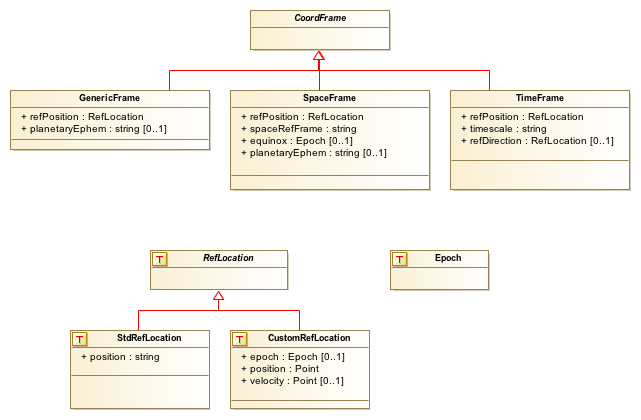
\includegraphics[width=4.5in]{diagrams/CoordFrame.png}
    \caption{Coordinate Frame elements}\label{fig:coordframe}
  \end{center}
  \end{figure}

  \subsection{CoordFrame (Abstract)}
  \label{sect:CoordFrame}
    This is the abstract, empty, base class for all coordinate frames. Coordinate frames provide metadata associated with the coordinate domain space. Typically, this will be related to the origin and orientation of the axes, but might include any metadata which pertains to the definition of the domain.

  \subsection{GenericFrame}
  \label{sect:GenericFrame}
    The generic coordinate frame is for cases where a domain-specific frame (e.g.: Space, Time), is not required, but the relevant reference metadata is still needed (e.g.: for Redshift or Spectral data)

    \subsubsection{GenericFrame.refPosition}
      \textbf{vodml-id: GenericFrame.refPosition} \newline
      \textbf{type: \hyperref[sect:RefLocation]{coords:RefLocation}} \newline
      \textbf{multiplicity: 1} \newline 
      Spatial location in phase space (position and velocity) at which the observed value is considered to have been taken. This will typically be given by a standard reference position, but we allow for custom locations as well.

    \subsubsection{GenericFrame.planetaryEphem}
      \textbf{vodml-id: GenericFrame.planetaryEphem} \newline
      \textbf{type: \hyperref[sect:ivoa]{ivoa:string}} \newline
      \textbf{multiplicity: 0..1} \newline 
      A planetary ephemeris MAY be provided, and SHOULD be provided whenever appropriate, to indicate which solar system ephemeris was used. If needed, but not provided, it is assumed to be "DE405"

  \subsection{SpaceFrame}
  \label{sect:SpaceFrame}
    A SpaceFrame is specified by its reference frame (orientation), and a reference position (origin). Currently only standard reference frames are allowed. An equinox MUST be provided for pre-ICRS reference frames. A planetary ephemeris MAY be provided if relevant. If needed, but not provided, it is assumed to be "DE405".

    \subsubsection{SpaceFrame.refPosition}
      \textbf{vodml-id: SpaceFrame.refPosition} \newline
      \textbf{type: \hyperref[sect:RefLocation]{coords:RefLocation}} \newline
      \textbf{multiplicity: 1} \newline 
      The spatial location at which the coordinates are considered to have been determined. This model supports locations provided as either a standard reference position (e.g. GEOCENTER), or a coordinate specifying a custom location (e.g. long, lat, height ).

    \subsubsection{SpaceFrame.spaceRefFrame}
      \textbf{vodml-id: SpaceFrame.spaceRefFrame} \newline
      \textbf{type: \hyperref[sect:ivoa]{ivoa:string}} \newline
      \textbf{vocabulary: http://www.ivoa.net/rdf/refframe} \newline
      \textbf{multiplicity: 1} \newline
      The spatial reference frame. Values MUST be selected from the controlled vocabulary at the given URL.

    \subsubsection{SpaceFrame.equinox}
      \textbf{vodml-id: SpaceFrame.equinox} \newline
      \textbf{type: \hyperref[sect:Epoch]{coords:Epoch}} \newline
      \textbf{multiplicity: 0..1} \newline 
      Reference date for the frame, required for pre-ICRS reference frames.

    \subsubsection{SpaceFrame.planetaryEphem}
      \textbf{vodml-id: SpaceFrame.planetaryEphem} \newline
      \textbf{type: \hyperref[sect:ivoa]{ivoa:string}} \newline
      \textbf{multiplicity: 0..1} \newline 
      Ephemeris file for solar system objects SHOULD be specified whenever relevant.


  \subsection{TimeFrame}
  \label{sect:TimeFrame}
    A TimeFrame SHALL include a time scale and reference position. It MAY also include a reference direction.

    \subsubsection{TimeFrame.refPosition}
      \textbf{vodml-id: TimeFrame.refPosition} \newline
      \textbf{type: \hyperref[sect:RefLocation]{coords:RefLocation}} \newline
      \textbf{multiplicity: 1} \newline 
      The spatial location at which the coordinate is considered to have been taken. This model supports locations provided as either a standard reference position (e.g. GEOCENTER), or a coordinate specifying a custom location (e.g. long, lat, height).

    \subsubsection{TimeFrame.timescale}
      \textbf{vodml-id: TimeFrame.timescale} \newline
      \textbf{type: \hyperref[sect:ivoa]{ivoa:string}} \newline
      \textbf{vocabulary: http://www.ivoa.net/rdf/timescale} \newline
      \textbf{multiplicity: 1} \newline
      The time scale sets the reference frame. The value MUST be selected from the controlled vocabulary at the given URL.

    \subsubsection{TimeFrame.refDirection}
      \textbf{vodml-id: TimeFrame.refDirection} \newline
      \textbf{type: \hyperref[sect:RefLocation]{coords:RefLocation}} \newline
      \textbf{multiplicity: 0..1} \newline 
      The reference direction is needed if the time stamps are transformed to a time frame with a different reference position. In those situations, the solar system ephemeris also comes into play. See: FITS WCS Paper IV for details, but in short: The reference direction, presumably the direction to the thing being observed, is used in conjunction with the reference position and planetary ephemeris to determine the correction applied for the path length change. To be fully useful, one also needs to know the location at which the observation was made ( i.e. the observatory location), which is not considered to be Frame metadata.


  \subsection{Epoch}
  \label{sect:Epoch}
  We define epoch as a primitive data type with the expected form "<type><year>" where type = "J" or "B" for Julian or Besselian respectively, and year is expressed as a decimal year. e.g.: "B1950", "J2000.0"


  \subsection{RefLocation (Abstract)}
  \label{sect:RefLocation}
    RefLocation defines the origin of the spatial coordinate space. This location is represented either by a standard reference position (for which the absolute location in phase space is known by definition), or a specified point in another Spatial frame. This object is used as the origin of the SpaceFrame here, but also to specify the Spatial Reference Position (refPosition) associated with other domain Frames. For example, in the Time domain, the Spatial Reference Position indicates that the 'time' values are the time that the 'event' occured at that location, which might be different from the detector location.


  \subsection{StdRefLocation}
  \label{sect:StdRefLocation}
    An absolute a-priori known location in phase space (position and velocity). Values are selected from the StdRefPosition vocabulary. Considering that the GEOCENTER is really the only place for which we know the absolute location at all times, all other locations require the specification of a planetary ephemeris. LSR[KD] are reserved for spectral and reshift frames. TOPOCENTER (location of the observer) is special in that it assumes that the observing location is available through other means (e.g. a geographic location or an orbit ephemeris). RELOCATABLE is available for simulations. UNKNOWN should only be used if absolutely necessary.

    \subsubsection{StdRefLocation.position}
      \textbf{vodml-id: StdRefLocation.position} \newline
      \textbf{type: \hyperref[sect:ivoa]{ivoa:string}} \newline
      \textbf{vocabulary: http://www.ivoa.net/rdf/refposition} \newline
      \textbf{multiplicity: 1} \newline
      Standard reference location. Values MUST be selected from the controlled vocabulary at the given URL.


  \subsection{CustomRefLocation}
  \label{sect:CustomRefLocation}
    A custom reference location in phase space (position and velocity). Position and velocity are given as coordinates with an associated SpaceFrame. An epoch MAY be provided to further refine the location.

    \subsubsection{CustomRefLocation.epoch}
      \textbf{vodml-id: CustomRefLocation.epoch} \newline
      \textbf{type: \hyperref[sect:Epoch]{coords:Epoch}} \newline
      \textbf{multiplicity: 0..1} \newline 
      Epoch for the reference location.

    \subsubsection{CustomRefLocation.position}
      \textbf{vodml-id: CustomRefLocation.position} \newline
      \textbf{type: \hyperref[sect:Point]{coords:Point}} \newline
      \textbf{multiplicity: 1} \newline 
      The spatial coordinates of the reference location.

    \subsubsection{CustomRefLocation.velocity}
      \textbf{vodml-id: CustomRefLocation.velocity} \newline
      \textbf{type: \hyperref[sect:Point]{coords:Point}} \newline
      \textbf{multiplicity: 0..1} \newline 
      The velocity of the reference location.


\pagebreak
\section{Coordinate Systems}

  % INSERT FIGURE HERE
  \begin{figure}[h]
  \begin{center}
    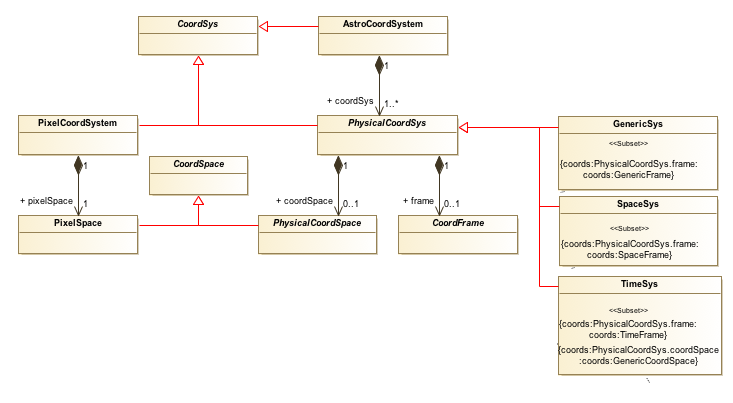
\includegraphics[width=5.25in]{diagrams/CoordSystems.png}
    \caption{Coordinate Systems }\label{fig:coordsys}
  \end{center}
  \end{figure}

  In the astronomical community, the term 'Coordinate System' is used to mean both ``the space in which a coordinate resides'', and ``a unique domain space'', folding in specific reference frame metadata.  In this model, we adopt the latter definition.  A Coordinate System provides a complete description of the domain space, including both the coordinate space description and associated Frame metadata.  To simplify the usage of these objects for the most common cases, we provide a set of standard CoordSpace instances which serve as defaults when not explicitely included in serializations.


  \subsection{CoordSys (Abstract)}
  \label{sect:CoordSys}
    Abstract head of the coordinate system object tree.


  \subsection{AstroCoordSystem}
  \label{sect:AstroCoordSystem}
    The AstroCoordSystem object holds a collection of component coordinate system descriptions across all represented physical domains.

    \subsubsection{AstroCoordSystem.coordSys}
      \textbf{vodml-id: AstroCoordSystem.coordSys} \newline
      \textbf{type: \hyperref[sect:PhysicalCoordSys]{coords:PhysicalCoordSys}} \newline
      \textbf{multiplicity: 1..*} \newline 
      Coordinate system description for each physical domain (Space, Time, etc).

  \subsection{PhysicalCoordSys (Abstract)}
  \label{sect:PhysicalCoordSys}
    Coordinate system description for any physical domain, such as Time, Space, Redshift, Temperature, Flux, etc.

    \subsubsection{PhysicalCoordSys.coordSpace}
      \textbf{vodml-id: PhysicalCoordSys.coordSpace} \newline
      \textbf{type: \hyperref[sect:PhysicalCoordSpace]{coords:PhysicalCoordSpace}} \newline
      \textbf{multiplicity: 0..1} \newline 
      Description of the coordinate space occupied by the property.

    \subsubsection{PhysicalCoordSys.frame}
      \textbf{vodml-id: PhysicalCoordSys.frame} \newline
      \textbf{type: \hyperref[sect:CoordFrame]{coords:CoordFrame}} \newline
      \textbf{multiplicity: 0..1} \newline 
      Associated Frame metadata.

  \subsection{PixelCoordSystem}
  \label{sect:PixelCoordSystem}
    The PixelCoordSystem provides a complete description of the pixel coordinate space. It SHALL contain one PixelSpace instance describing each pixel axis.

    \subsubsection{PixelCoordSystem.pixelSpace}
      \textbf{vodml-id: PixelCoordSystem.pixelSpace} \newline
      \textbf{type: \hyperref[sect:PixelSpace]{coords:PixelSpace}} \newline
      \textbf{multiplicity: 1} \newline 
      The pixel space completely defines the pixel coordinate axes.  Each axis MUST be defined as a BinnedAxis type.

  \subsection{GenericSys}
  \label{sect:GenericSys}
    Specialized coordinate system for generic, one-dimensional domains not covered by other, more concrete objects. If a CoordSpace is not provided, it is assumed to be represented by a Standard 1-Dimensional Coordinate Space as described in Appendix B.

    \noindent \textbf{subset} \newline
    \indent   \textbf{role: coords:PhysicalCoordSys.frame} \newline
    \indent   \textbf{type: coords:GenericFrame} \newline


  \subsection{SpaceSys}
  \label{sect:SpaceSys}
    Specialized coordinate system for the Spatial domain. This object SHOULD include an appropriate SpaceFrame. In Appendix B, we define two standard spatial coordinate space instances (Spherical and Cartesian), which may be referenced in serializations. If a CoordSpace is not provided, it is assumed to be represented by a Standard Spherical Coordinate Space.

    \noindent \textbf{subset} \newline
    \indent   \textbf{role: coords:PhysicalCoordSys.frame} \newline
    \indent   \textbf{type: coords:SpaceFrame} \newline


  \subsection{TimeSys}
  \label{sect:TimeSys}
    Specialized coordinate system for the Temporal domain. This object SHOULD include an appropriate TimeFrame. If a CoordSpace is not provided, it is assumed to be represented by a Standard 1-Dimensional Coordinate Space as described in Appendix B.

    \noindent \textbf{subset} \newline
    \indent   \textbf{role: coords:PhysicalCoordSys.frame} \newline
    \indent   \textbf{type: coords:TimeFrame} \newline


    \noindent \textbf{subset} \newline
    \indent   \textbf{role: coords:PhysicalCoordSys.coordSpace} \newline
    \indent   \textbf{type: coords:GenericCoordSpace} \newline


\pagebreak
\section{Coordinate Space}

  % INSERT FIGURE HERE
  \begin{figure}[h]
  \begin{center}
    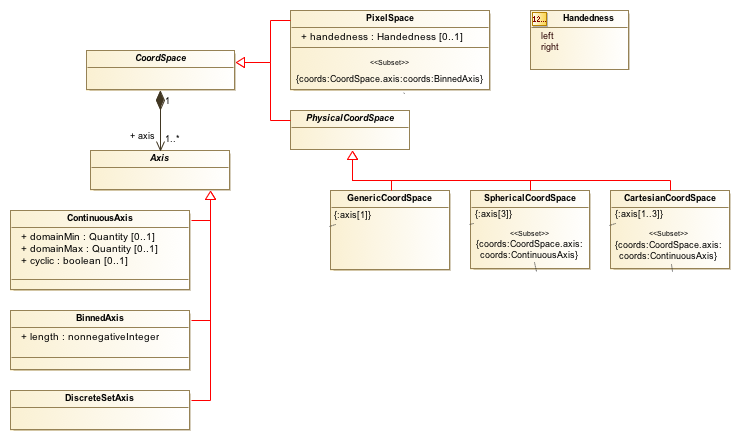
\includegraphics[width=5.25in]{diagrams/CoordSpace.png}
    \caption{Coordinate Spaces}\label{fig:coordspace}
  \end{center}
  \end{figure}

  \subsection{CoordSpace (Abstract)}
  \label{sect:CoordSpace}
    This object defines a domain space. i.e.: it describes the set of possible coordinate values.

    \subsubsection{CoordSpace.axis}
      \textbf{vodml-id: CoordSpace.axis} \newline
      \textbf{type: \hyperref[sect:Axis]{coords:Axis}} \newline
      \textbf{multiplicity: 1..*} \newline 
      Describes an axis of the coordinate space.


  \subsection{Axis (Abstract)}
  \label{sect:Axis}
    The abstract parent class for all coordinate axis types. We provide concrete classes for the most common types of data, Continuous, Binned, and Discrete, but allow extension for other types as needed.

    \subsubsection{Axis.name}
      \textbf{vodml-id: Axis.name} \newline
      \textbf{type: \hyperref[sect:ivoa]{ivoa:string}} \newline
      \textbf{multiplicity: 0..1} \newline 
      Freeform string, provides the name or label for the axis.

  \subsection{ContinuousAxis}
  \label{sect:ContinuousAxis}
    Axis description for continuous data. This object describes the domain for a particular axis of the domain space. It allows for the specification of the legal domain range (min,max), and a flag indicating if the axis is cyclic.

    \subsubsection{ContinuousAxis.domainMin}
      \textbf{vodml-id: ContinuousAxis.domainMin} \newline
      \textbf{type: \hyperref[sect:ivoa]{ivoa:Quantity}} \newline
      \textbf{multiplicity: 0..1} \newline 
      Minimum extent of the axis domain space. If not provided, the domain space is considered to have no lower bound (-INFINITY).

    \subsubsection{ContinuousAxis.domainMax}
      \textbf{vodml-id: ContinuousAxis.domainMax} \newline
      \textbf{type: \hyperref[sect:ivoa]{ivoa:Quantity}} \newline
      \textbf{multiplicity: 0..1} \newline 
      Maximum extent of the axis domain space. If not provided, the domain space is considered to have no upper bound (+INFINITY).

    \subsubsection{ContinuousAxis.cyclic}
      \textbf{vodml-id: ContinuousAxis.cyclic} \newline
      \textbf{type: \hyperref[sect:ivoa]{ivoa:boolean}} \newline
      \textbf{multiplicity: 0..1} \newline 
      Flag indicating if the axis is cyclic in nature. If not provided, it is assumed to be FALSE.

  \subsection{BinnedAxis}
  \label{sect:BinnedAxis}
    Axis description for binned data, where values along the axis correspond to a bin number.

    \subsubsection{BinnedAxis.length}
      \textbf{vodml-id: BinnedAxis.length} \newline
      \textbf{type: \hyperref[sect:ivoa]{ivoa:nonnegativeInteger}} \newline
      \textbf{multiplicity: 1} \newline 
      The length, or number of bins, along the axis.

  \subsection{DiscreteSetAxis}
  \label{sect:DiscreteSetAxis}
    Axis type specifically intended for enumerated coordinates. Since the content and nature of this axis type is heavily dependent on the use case, we define no additional metadata here. Extensions of this type may include additional metadata relevant to the particular use cases. For example, an extension could include the allowed set of values.


  \subsection{PhysicalCoordSpace (Abstract)}
  \label{sect:PhysicalCoordSpace}
    Abstract head of coordinate spaces related to physical properties.


  \subsection{SphericalCoordSpace}
  \label{sect:SphericalCoordSpace}
    Spatial domain, three-dimensional spherical coordinate space. The particulars of the axis descriptions depend on the flavor of space being instantiated. In Appendix B., we provide a Standard Spherical Coordinate Space instance which applies to many Astronomical use cases. It provides the default space for SpaceSys instances, and may be referenced in serializations.

    \noindent \textbf{subset} \newline
    \indent   \textbf{role: coords:CoordSpace.axis} \newline
    \indent   \textbf{type: coords:ContinuousAxis} \newline


    \noindent \textbf{constraint} \newline
    \indent    \textbf{detail: SphericalCoordSpace.axis[3] }\newline


  \subsection{CartesianCoordSpace}
  \label{sect:CartesianCoordSpace}
    Spatial domain, three-dimensional cartesian coordinate space. The particulars of the axis descriptions depend on the physical constraints of the instance. In Appendix B, we provide the description of a Standard Cartesian Coordinate Space instance which applies to many Astronomical cases, and may be referenced in serializations.

    \noindent \textbf{subset} \newline
    \indent   \textbf{role: coords:CoordSpace.axis} \newline
    \indent   \textbf{type: coords:ContinuousAxis} \newline


    \noindent \textbf{constraint} \newline
    \indent    \textbf{detail: CartesianCoordSpace.axis[1..3] }\newline


  \subsection{GenericCoordSpace}
  \label{sect:GenericCoordSpace}
    Generic, one-dimensional coordinate space suitable for use with most non-spatial properties. In Appendix B, we provide the description of a Standard 1D Coordinate Space instance which may be referenced in serializations.

    \noindent \textbf{constraint} \newline
    \indent    \textbf{detail: GenericCoordSpace.axis[1] }\newline


  \subsection{PixelSpace}
  \label{sect:PixelSpace}
  The Pixel coordinate space is defined as a 'virtual' binned space, with no physical meaning. The axes in this space provide integer indices into that space.  A PixelSpace SHALL include one or more BinnedAxis objects describing the pixel coordinate space. A handedness value MAY be provided to specify the relative orientation of the axes.

    \noindent \textbf{subset} \newline
    \indent   \textbf{role: coords:CoordSpace.axis} \newline
    \indent   \textbf{type: coords:BinnedAxis} \newline


    \subsubsection{PixelSpace.handedness}
      \textbf{vodml-id: PixelSpace.handedness} \newline
      \textbf{type: \hyperref[sect:Handedness]{coords:Handedness}} \newline
      \textbf{multiplicity: 0..1} \newline 
      Specifies the handedness of the coordinate space.


  \subsection{Handedness}
  \label{sect:Handedness}

  The handedness of a coordinate space. For most cases, this will be a fixed value in the specification of the coordinate space. We provide this element to allow this flexibility when needed. In this document, it is used in the Pixel domain.

  \noindent \underline{Enumeration Literals}
  \vspace{-\parsep}
  \small
  \begin{itemize}
  
    \item[\textbf{left}]: \textbf{vodml-id:} Handedness.left \newline
          \textbf{description:} positive x and y axes point right and up, the positive z axis points inward
    \item[\textbf{right}]: \textbf{vodml-id:} Handedness.right \newline
          \textbf{description:} positive x and y axes point right and up, the positive z axis points outward
  \end{itemize}
  \normalsize



\appendix
% Use Cases and Requirements
\pagebreak
\section{Requirements Mapping}
\label{sect:req_map}

The table below provides a mapping of the various elements of this model to requirements served by that object.

% The following is generated from the list of vo-dml IDs at the bottom of the vo-dml.html documentation
\small
\begin{longtable}[l]{|l|l|}
  \hline
  \textbf{vodml-id} & \textbf{pertains to}    \\
  \hline
  \endfirsthead
  \hline
  \textbf{vodml-id} & \textbf{pertains to}    \\
  \hline
  \endhead

%==== HERE =====
        AstroCoordSystem                  & coords.008, coords.010                      \\
%       AstroCoordSystem.coordSys         &                                             \\
        Axis                              & coords.001.1, coords.001.2                  \\
%       Axis.name                         &                                             \\
        BinnedAxis                        & dom.002.1, coords.001.2                     \\
        BinnedAxis.length                 & coords.001.3                                \\
        BinnedCoordinate                  & coords.006                                  \\
%       BinnedCoordinate.cval             &                                             \\
        CartesianCoordSpace               & user.002                                    \\
        ContinuousAxis                    & dom.002.2, dom.002.3, coords.001.2          \\
        ContinuousAxis.cyclic             & coords.001.3                                \\
        ContinuousAxis.domainMax          & coords.001.3                                \\
        ContinuousAxis.domainMin          & coords.001.3                                \\
        CoordFrame                        & coords.002, coords.004                      \\
        Coordinate                        & user.001, coords.003, coords.007            \\
        Coordinate.coordSys               & user.001, coords.004                        \\
        CoordSpace                        & coords.001                                  \\
%       CoordSpace.axis                   &                                             \\
        CoordSys                          & coords.008                                  \\
        CustomRefLocation                 & dom.002.2, coords.002                       \\
%       CustomRefLocation.epoch           &                                             \\
%       CustomRefLocation.position        &                                             \\
%       CustomRefLocation.velocity        &                                             \\
        DiscreteSetAxis                   & dom.002.4, coords.001.2                     \\
        Epoch                             & dom.002.2, coords.001.2                     \\
        GenericCoordSpace                 & user.002                                    \\
        GenericSys                        & user.002                                    \\
        GenericFrame                      & coords.002                                  \\
%       GenericFrame.planetaryEphem       &                                             \\
%       GenericFrame.refPosition          &                                             \\
        Handedness                        & coords.001                                  \\
%       Handedness.left                   &                                             \\
%       Handedness.right                  &                                             \\
        ISOTime                           & user.002, coords.006                        \\
%       ISOTime.date                      &                                             \\
        JD                                & user.002, coords.006                        \\
%       JD.date                           &                                             \\
        MJD                               & user.002, coords.006                        \\
%       MJD.date                          &                                             \\
        PhysicalCoordinate                & user.001, user.002, dom.001, coords.003, coords.005, coords.006 \\
%       PhysicalCoordinate.cval           &                                             \\
        PhysicalCoordSpace                & coords.001                                  \\
        PhysicalCoordSys                  & dom.001, coords.001, coords.002             \\
%        PhysicalCoordSys.coordSpace       & dom.001, coords.001                        \\
%        PhysicalCoordSys.frame            & dom.001, coords.002                        \\
        PixelCoordSystem                  & dom.002.1, coords.008                       \\
        PixelCoordSystem.pixelSpace       & dom.002.1, coords.008, coords.009           \\
        PixelIndex                        & dom.002.1, coords.003, coords.005           \\
        PixelSpace                        & dom.002.1, coords.001.1                     \\
%       PixelSpace.handedness             &                                             \\
        Point                             & dom.002.2, user.001, user.002, coords.003, coords.005, coords.006, coords.007     \\
%       Point.axis1                       & coords.007                       \\
%       Point.axis2                       & coords.007                       \\
%       Point.axis3                       & coords.007                       \\
        PolCoordinate                     & dom.002.4, coords.005              \\
        PolState                          & dom.002.4, coords.003                       \\
%       PolState.cval                     &                                             \\
%       PolStateEnum                      &                                             \\
        RefLocation                       & dom.002.2, coords.002                       \\
        SpaceFrame                        & dom.002.2, coords.002                       \\
%       SpaceFrame.equinox                &                                             \\
%       SpaceFrame.planetaryEphem         &                                             \\
%       SpaceFrame.refPosition            &                                             \\
%       SpaceFrame.spaceRefFrame          &                                             \\
        SpaceSys                          & user.002                                    \\
        SphericalCoordSpace               & user.002                                    \\
        StdRefLocation                    & dom.002.2, coords.002                       \\
%       StdRefLocation.position           &                                             \\
        TimeFrame                         & dom.002.3, coords.002                       \\
%       TimeFrame.refDirection            &                                             \\
%       TimeFrame.refPosition             &                                             \\
%       TimeFrame.timescale               &                                             \\
        TimeInstant                       & dom.002.3                                   \\
        TimeOffset                        & dom.002.3, user.002, coords.006             \\
%       TimeOffset.time                   &                                             \\
%       TimeOffset.time0                  &                                             \\
        TimeStamp                         & dom.002.3, user.002, coords.003, coords.005, coords.007 \\
        TimeSys                           & user.002                                    \\

  \hline
\end{longtable}
\normalsize


% Standard Coordinate Spaces
\pagebreak
\section{Standard Coordinate Spaces}
\label{sect:StdCoordSpaces}
We provide standard instances of commonly used coordinate spaces as instances of elements from this model.  Each element has a formal identifier (ID) which can be used to reference the instance given here.

  \subsection{Standard Cartesian Coordinate Space}
  \label{sect:Cartesian}

  \begin{minipage}{0.5\textwidth}
    \small
    \textbf{id}: \_CARTESIAN\_CoordSpace \newline
    Coordinate space comprised of 3 orthogonal axes.
    
    \noindent \textbf{Axis1} \newline
    \indent id:  \_CARTESIAN\_X\_Axis \newline
    \indent domainMin:  -Infinity \newline
    \indent domainMax:  +Infinity \newline
    \indent cyclic:  False \newline
    
    \noindent \textbf{Axis2} \newline
    \indent id:  \_CARTESIAN\_Y\_Axis \newline
    \indent domainMin:  -Infinity \newline
    \indent domainMax:  +Infinity \newline
    \indent cyclic:  False \newline
    
    \noindent \textbf{Axis3} \newline
    \indent id:  \_CARTESIAN\_Z\_Axis \newline
    \indent domainMin:  -Infinity \newline
    \indent domainMax:  +Infinity \newline
    \indent cyclic:  False \newline
    \normalsize
  \end{minipage}
  \begin{minipage}{0.5\textwidth}
    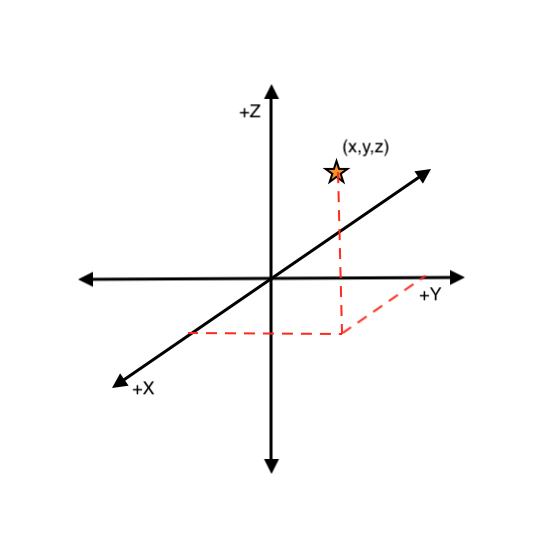
\includegraphics{diagrams/CartesianSpace.png}
  \end{minipage}
  \vspace{-0.75cm}

  \subsection{Standard Spherical Coordinate Space}
  \label{sect:Spherical}

  \begin{minipage}{0.5\textwidth}
    \small
    \textbf{id}: \_SPHERICAL\_CoordSpace \newline
    A 3 dimensional spherical coordinate space, comprised of 2 angular axes and 1 radial axis.
    
    \noindent \textbf{Axis1} \newline
    \indent id:  \_SPHERICAL\_Lat\_Axis \newline
    \indent domainMin:  -90.0 deg \newline
    \indent domainMax:  +90.0 deg \newline
    \indent cyclic: False \newline
    
    \noindent \textbf{Axis2} \newline
    \indent id:  \_Spherical\_Long\_Axis \newline
    \indent domainMin: 0.0 deg \newline
    \indent domainMax: 360.0 deg \newline
    \indent cyclic: True \newline
    
    \noindent \textbf{Axis3} \newline
    \indent id:  \_Spherical\_R\_Axis \newline
    \indent domainMin: 0.0 \newline
    \indent domainMax: +Infinity \newline
    \indent cyclic:  False \newline
    \normalsize
  \end{minipage}
  \begin{minipage}{0.5\textwidth}
    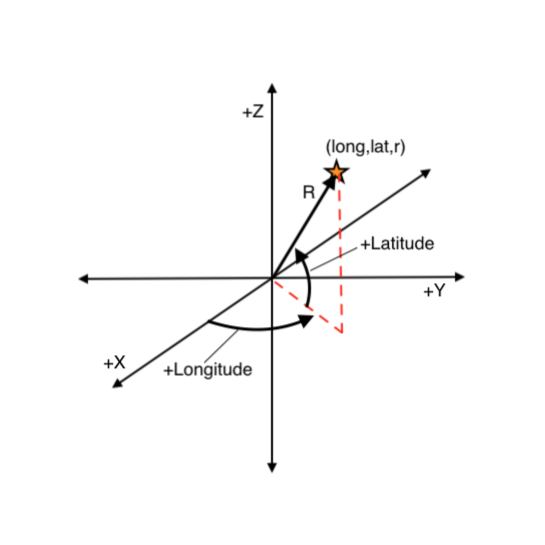
\includegraphics{diagrams/SphericalSpace.png}
  \end{minipage}

  \subsection{Standard 1D Coordinate Space}
  \label{sect:1DSpace}

  \vspace{-3cm}
  \begin{minipage}{0.5\textwidth}
    \small
    \textbf{id}: \_STANDARD\_1D\_CoordSpace \newline
    Coordinate space comprised of 1 axis.
    
    \noindent \textbf{Axis1} \newline
    \indent id:  Standard\_1D\_Axis \newline
    \indent domainMin:  -Infinity \newline
    \indent domainMax:  +Infinity \newline
    \indent cyclic:  False \newline
    
    \normalsize
  \end{minipage}
  \begin{minipage}{0.5\textwidth}
    
\includegraphics{diagrams/Standard1DSpace.png}
  \end{minipage}



% Vocabularies defined by the model
\pagebreak
\section{Standard Vocabularies}
Quick reference to standard vocabularies used in this model.

  \begin{enumerate}
    \item \textbf{Standard Reference Frame (StdRefFrame)}
    \begin{itemize}
      \item[BaseURL:] http://www.ivoa.net/rdf
      \item[Vocabulary:] refframe
    \end{itemize}
    \item \textbf{Standard Reference Frame (StdRefPos)}
    \begin{itemize}
      \item[BaseURL:]  http://www.ivoa.net/rdf
      \item[Vocabulary:] refposition
    \end{itemize}
    \item \textbf{Standard Reference Frame (StdTimeScale)}
    \begin{itemize}
      \item[BaseURL:]  http://www.ivoa.net/rdf
      \item[Vocabulary:] timescale
    \end{itemize}
\end{enumerate}



% Changes from previous version
\pagebreak
\section{Changes from Previous Versions}

%No previous versions yet.  

% these would be subsections "Changes from v. WD-..."
% Use itemize environments.
\subsection{Changes from WD-2019-03-20}
\begin{itemize} 
  \item Section 1.2: added clarifying text on the distinction between Quantity, Coordinate, and Measurement in the IVOA models.
  \item Updated URLs for vocabularies
  \item Appendix B: changed 'Class' to 'ObjectType' to better align with the VO-DML description.
  \item Appendix C: brought initial vocabulary content in line with URL content.
\end{itemize}
\subsection{Changes from PR-2019-08-30}
\begin{itemize} 
  \item Migrate CoordSys element to include both CoordSpace and CoordFrame concepts.
  \item Coordinate element to reference CoordSys, rather than CoordFrame and CoordSpace.axis
  \item Removed specialized Coordinate types linked to standard spatial coordinate spaces, replace with Point
  \item Corrected multiplicity of SpaceFrame.planetaryEphem
  \item Corrected URLs for vocabularies ('http' not 'https')
  \item Corrected LaTex for TCG and TCB records to fix display 
\end{itemize}
\subsection{Changes from PR-2020-03-10}
\begin{itemize} 
  \item Restored Point subclasses: CartesianPoint, LonLatPoint, GenericPoint
  \item Removed 'default' listing of dependent vocabularies from Appendices.
  \item Update citation tags for IVOA standards.
  \item Revision to the Use Case section in response to RFC comments.
\end{itemize}


% Appendix for UML diagram conventions
\pagebreak
\section{Modeling Conventions}
This model follows the VO-DML modeling practices, however, the UML representations may vary depending on the tool used.  Below we describe the graphical representation of the modeling concepts and relations.

  \begin{figure}[h]
  \begin{center}
    \fbox{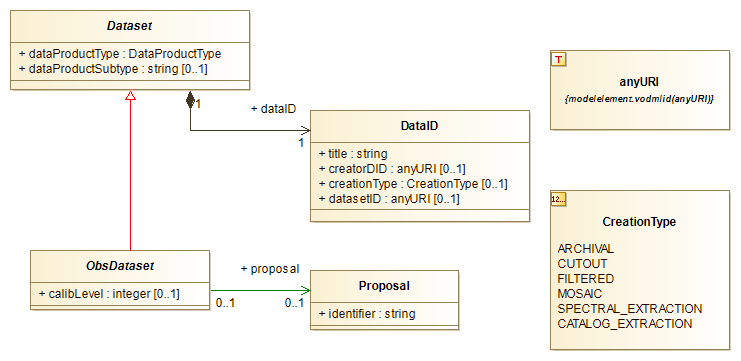
\includegraphics[width=0.9\textwidth]{diagrams/notation_example.png}}
    \caption{Notation example diagram}\label{fig:notation_example}
  \end{center}
  \end{figure}

  \subsection{ObjectType}
  \label{sect:ObjectType}
  ObjectTypes are represented by a plain box. The type name is annotated in the top window, abstract
types use italic typeface. Attributes, if any, are listed in the lower panel. Attributes may only be
of primitive type (real, string, etc), a defined DataType, or an Enumeration type. Relationships to
other objects are defined via the composition and reference relation arrows.

  \subsection{DataType}
  \label{sect:DataType}
  DataTypes are represented by a box shape similar to ObjectType, but annotated with a "T" symbol in the top left corner.

  \subsection{Enumerations}
  \label{sect:Enumerations}
  Enumerations are represented by a box shape similar to ObjectType, but annotated with a "1,2.."
symbol in the top left corner. Enumeration Literals (possible values) are listed below the
enumeration type name.

  \subsection{Generalization}
  \label{sect:Generalization}
  Generalizations are represented by a red line, with open triangle at the end of the source, or more general, object.

  \subsection{Composition}
  \label{sect:Composition}
  The composition relation is indicated by a black line with a solid diamond attached to the
containing object, and an arrow pointing to the object being contained. The composition relation is
very tight, where the container is responsible for the creation and existence of the target. Any
object may be in no more than one composition relation with any container. The attribute name
for the composition relation is annotated at the destination of the relation (e.g. "+ dataID"). This is
typically a lower-cased version of the destination type name, but this is not required.

  \subsection{Reference}
  \label{sect:Reference}
  The reference relation is indicated by a green line, with an arrow pointing to the object being
referenced. The reference relation is much looser than composition, the container has no
ownership of the target, but merely holds a pointer, or other indirect connection to it. The
attribute name is annotated at the destination of the relation ( e.g. "+ proposal"). This is typically
a lower-cased version of the destination type name, but may be another name indicating the role
that the element is playing in this context.

  \subsection{Multiplicity}
  \label{sect:Multiplicity}
  All attributes and relations have a multiplicity associated with them. For attributes, the multiplicity
is contained within brackets just after the attribute name. If no bracket is displayed, this is
equivalent to '[1]'.
\begin{itemize}
\item 1 = one and only one value must be provided.
\item 0..1 = zero or one value may be provided.
\item * = zero or more values may be provided (open ended).
\end{itemize}



% Appendix for IVOA Base types
\pagebreak
\section{Data Types}

  \subsection{Base Data Types}
  \label{sect:ivoa}
  Provides a set of standardized primitive data types as well as types for representing quantities
( values with associated units ). We provide a diagram of the model here, and refer the reader to
Section 5 of the VO-DML modeling specification document \citep{2018ivoa.spec.0910L} for more information.


    \begin{figure}[h]
    \begin{center}
      \fbox{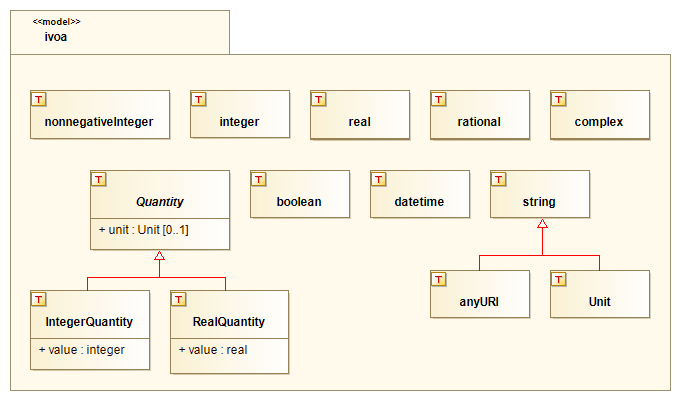
\includegraphics[width=\textwidth-0.1in]{diagrams/ivoa_types.png}}
      \caption{Base Data Types}\label{fig:basetypes}
    \end{center}
    \end{figure}


  \subsubsection{Units}
  \label{sect:Units}
  This model requires the use of the IVOA VOUnits Standard \citep{2014ivoa.spec.0523D} for representing units of physical
quantities. This standard reconciles common practices and current standards for use within the
IVOA community.

  \subsubsection{Dates}
  \label{sect:Dates}
  The 'datetime' datatype is for expressing date-time values. The string representation of a
datetime value should follow the FITS convention for representing dates. The FITS standard is
effectively ISO8601 format without the "Z" tag to indicate UTC (YYYY-MM-DDThh:mm:ss).
Values are nominally expressed in UTC.


\bibliography{ivoatex/ivoabib,ivoatex/docrepo,other}

\end{document}
